\chapter{Geoteknik}

For at kunne dimensionere et fundament, er det vigtigt at have en grundlæggende viden om det materiale, der arbejdes med, altså jord, samt dets egenskaber og styrkeegenskaber. I det følgende vil der derfor foretages en beskrivelse af jord og dets styrkeparametre.
\newline \indent{     }  Efterfølgende….

\section{Jord}

HER INDSÆTTES JORD-DELEN (som Michael er ved at skrive)

\section{Fundering}
De to mest almindelige funderingsmetoder er pælefundering og direkte fundering.
\newline \indent{     }  Ved direkte fundering hviler fundamentet direkte på terrænet. 
\newline \indent{     }  Ved pælefundering er søjleformede pæle af træ, beton, og/eller stål, rammet, presset, vibreret eller udstøbt i jorden. Pæleformen er normalt cylindrisk med cirkulært eller kvadratisk tværsnit \citep[ s. 355]{geoteknik}.
Ligesom ved direkte fundering er formålet med pælefundering og pælene at overføre belastningen fra overbygningen og ned til det bæredygtige jordlag. 
\newline
\newline
Valg af funderingsmetode afhænger af jordbunds- og grundvandsforhold samt de belastninger, som konstruktionen er udsat for \citep[ s. 355]{geoteknik}. Det er derfor nødvendigt at have kendskab til områdets geologi, og at tolke på de boreprofiler, der bliver udført på stedet. 

\section{Antagelser}
Idét Aalborg er funderet på meget blødt ler, benyttes boreprofiler fra Hals/Hou, og det antages, at disse boreprofiler er fra området ved Strøybergs Palæ. 
\newline \indent{     }  Forsøgene er udført på baskarpsand fra Sverige, hvilket antages at være sandet fra boreprofilerne.

\section{Forsøg}
For at bestemme styrkeparametre for jorden udføres laboratorieforsøg, som bruges ved dimensionering af fundamentet.
\newline
\newline
Formålet med forsøgene er at bestemme friktionsvinklen, ved: 

\begin{center}
	$\varphi_{tr} = 30^\circ - \frac{3}{U} + (14 - \frac{4}{U}) I_D$
\end{center}

\begin{itemize}
	\item[-] U: Uensformighedtal
	\item[-] $I_D$: Relativ lejringstæthed
\end{itemize}

Friktionsvinklen $\varphi$ er et mål for jords styrke, og skønnes ud fra sigteanalyse samt løs og fast lejring. Ved hjælp af nedenstående fire forsøg bestemmes friktionsvinklen, idet uensformighedstallet og den relative lejringstæthed bestemmes herudfra: 
\begin{enumerate}
	\item Vandindhold
	\item Sigteanalyse
	\item Kornvægtfylde
	\item Løs og fast lejring
\end{enumerate}
Tabeller over resultater, fremgangsmåde, apparaturliste samt fejlkilder for de enkelte forsøg, findes i bilag A-D.

\subsection{Forsøg 1: Vandindhold}
Formålet med forsøget “vandindhold” er at finde vandindholdet \textit{w} i jordprøven. Vandindholdet er defineret som jordens vægttab i \% af tørvægten ved tørring i et varmeskab ved en temperatur på 105 grader. For naturligt forekommende jordarter kan vandindholdet ligge mellem nul og flere hundrede procent.
\newline
\newline
Vandindholdet beregnes ved:

\begin{center}
	$w = \frac{Vandvægt}{Kornvægt} = \frac{W_w}{W_s}\cdot 100\% = \frac{(W+sk)-(W_s+sk)}{(W_s+sk)-sk}\cdot 100\%$
\end{center}

\begin{itemize}
	\item[-] $W_w$: Vægten af vandet i prøven [g]
	\item[-] $W_s$: Vægten af det tørrede materiale [g]
	\item[-] W: Vægten af prøven før tørring [g]
	\item[-] sk: Vægten af skålen [g]
\end{itemize}

Forsøget er udført to gange. Vandindholdet for de to forsøg er beregnet til:

\begin{center}
	$w_1 = \frac{81,\!02 g - 80,\!99 g}{80,\!99 g - 3,\!07 g}\cdot 100\% = 0,\!04\%$
\end{center}

\begin{center}
	$w_2 = \frac{89,\!83 g - 89,\!79}{89,\!79 g - 3,\!11 g}\cdot 100\% = 0,\!05\%$
\end{center}

Til videre beregninger benyttes gennemsnittet for vandindholdet for forsøg 1 og forsøg 2, som er $0,\!04$\%.. Dette skal bruges som et rent tal, som er $,\!0004$. 
\newline
\newline
MANGLER KONKLUSION.....

\subsection{Forsøg 2: Sigteanalyse}
Formålet med “sigteanalyse” er at bestemme jordkornenes vægtmæssige fordeling efter størrelse i sand- og grusfraktion, for at beregne uensformighedstallet \textit{U} for jorden:

\begin{center}
	$U = \frac{d_{60}}{d_{10}}$
\end{center}

\begin{itemize}
	\item[-] $d_{60}$: 60\%-fraktilen
	\item[-] $d_{10}$: 10\%-fraktilen
\end{itemize}

Uensformighedstallet fortæller, hvor velsorteret jorden er:

\begin{itemize}
	\item[-] Velsorteret: $U < 2$
	\item[-] Sorteret: $2 < U < 3,\!5$
	\item[-] Ringe sorteret: $3,\!5 < U < 7$
	\item[-] Usorteret: $U > 7$
\end{itemize}

Forsøget er udført to gange, og der er derfor lavet en sigtekurve for hvert forsøg, og uensformighedstallet er udregnet for begge forsøg. 
\newline \indent{     }  Det procentvise gennemfald i hver sigte er beregnet, og herudfra fås nedenstående sigtekurver: 

\begin{figure}[htbp] \centering
	\begin{minipage}[b]{0.48\textwidth}\centering
		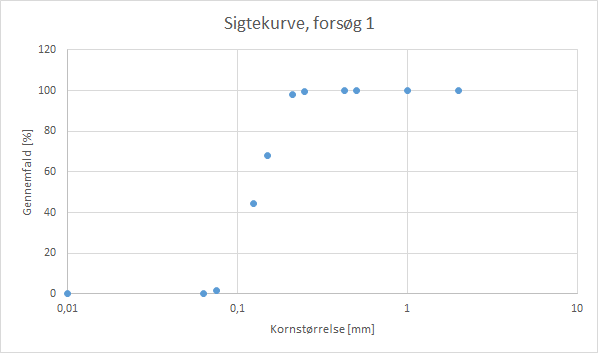
\includegraphics[width=1.0\textwidth]{billeder/sigtekurve1.png}
		\caption{Sigtekurve til forsøg 1}
		\label{fig:sigtekurve1}
	\end{minipage}\hfill
	\begin{minipage}[b]{0.48\textwidth}\centering
		\centering
		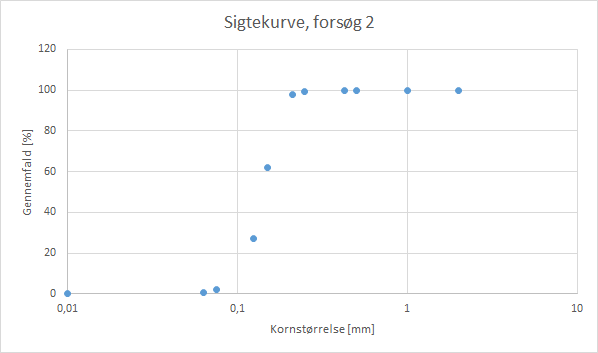
\includegraphics[width=1.0\textwidth]{billeder/sigtekurve2.png}
		\caption{Sigtekurve til forsøg 2}
		\label{fig:sigtekurve2}
	\end{minipage}
\end{figure}

Uensformighedstallet for begge forsøg er beregnet, ved at lave lineær regression i mellem henholdsvis 10\% og 60\% og derved finde 10\%-fraktilen og 60\%-fraktilen.
\newline
\newline
Ved forsøg 1 er 10\%-fraktilen og 60\%-fraktilen beregnet til: 
\begin{center}
	$d_{10} = 0,\!08$ og $d_{60} = 0,\!14$
\end{center} 

Uensformighedstallet i forsøg 1 er hermed:
\begin{center}
	$U = \frac{0,\!14}{0,\!08} = 1,\!67$
\end{center}

Ved forsøg 2 er 10\%-fraktilen og 60\%-fraktilen beregnet til:
\begin{center}
	$d_{10} = 0,\!91$ og $d_{60} = 0,\!15$
\end{center} 

Uensformighedstallet i forsøg 2 er hermed:
\begin{center}
	$U = \frac{0,\!15}{0,\!91} = 1,\!64$
\end{center}

Til videre beregninger benyttes gennemsnittet af uensformighedstallet for forsøg 1 og forsøg 2, som er $1,\!65$. Dette tal fortæller, at jorden er velsorteret. 

\subsection{Forsøg 3: Kornvægtfylde}
Formålet med “kornvægtfylde” er at finde den relative densitet $d_s$, også kaldet kornvægtfylden, for jordprøven. For jordarter uden organisk indhold kan kornvægtfylden variere fra $2,\!65$ for rent kvartsand til $2,\!85$ for visse lermineraler. I dette forsøg søges altså et resultat der ligger så tæt på $2,\!65$ som muligt.
\newline
\newline
Kornvægtfylden beregnes ved:

\begin{center}
	$d_s = \frac{W_s p_w^t}{W_s + W_2 - W_1}$
\end{center}

\begin{itemize}
	\item[-] $W_s$: Vægten at tørt kornmateriale [g]
	\item[-] $p_w^t$: Densitet af demineraliseret vand ved målte temperatur $[\frac{g}{cm^3}]$
	\item[-] $W_2$: Vægten af pyknometeret fyldt med demineraliseret vand [g]
	\item[-] $W_1$: Vægten af pyknometer fyldt med prøve og demineraliseret vand [g]
\end{itemize}

Forsøget er udført to gange. Kornvægtfylden for de to forsøg er beregnet til:

\begin{center}
	Forsøg 1: $d_{s} = \frac{161,\!27 g \cdot 0,\!998 \frac{g}{mL}}{161,\!27 g + 641,\!16 g - 728,\!89 g} = 2,\!19 \frac{g}{m^3}$
\end{center}
\begin{center}
	Forsøg 2: $d_{s} = \frac{150,\!06 g \cdot 0,\!998 \frac{g}{mL}}{150,\!06 g + 615,\!97 g - 709,\!40 g} = 2,\!64 \frac{g}{m^3}$
\end{center} 

Resultatet fra forsøg 2 anvendes til videre beregninger, fordi resultatet fra forsøg 1 vurderes til at være for langt fra den ønskede værdi på $2,\!65$.

\subsection{Forsøg 4: Løs og fast lejring}
Formålet med “løs og fast lejring” er finde jordens relative lejringstæthed $I_D$. Lejringstætheden er et tal som vokser fra 0 til 1, når lejringstætheden varierer fra den løseste til den fasteste lejring.
\newline
\newline
$I_D$ bestemmes ved:

\begin{center}
	$I_D = \frac{e_{max} - e_{in situ}}{e_{max} - e_{min}}$
\end{center}

\begin{itemize}
	\item[-] $e_{min}$: jordens gennemsnitlige poretal for den fasteste lejring 
	\item[-] $e_{max}$: jordens gennemsnitlige poretal for den løseste lejring
	\item[-] $e_{in situ}$: jordens naturlige poretal 
\end{itemize}

Poretallet \textit{e}, for henholdsvis den løseste og fasteste lejring beregnes ved:

\begin{center}
	$e = \frac{d_s \rho_w  V}{W_s} - 1$
\end{center}

\begin{itemize}
	\item[-] $d_s$: kornvægtfylde [rent tal], som er fundet i forsøg 3: kornvægtfylde, til $2,\!64 \frac{g}{m^3}$ 
	\item[-] $\rho_w$: Vands densitet på $1 \frac{g}{cm^3}$
	\item[-] V: Volumen af materialet $[cm^3]$
	\item[-] $W_s$: Vægten at tørt kornmateriale [g]
\end{itemize}

Der er udført fire forsøg for henholdsvis den løseste og den fasteste lejring, hvor jordens gennemsnitlige poretal er beregnet til:

\begin{center}
	$e_{min} = \frac{0,\!595 + 0,\!571 + 0,\!573 + 0,\!569}{4} = 0,\!577$
\end{center}

\begin{center}
	$e_{max} = \frac{0,\!873 + 0,\!875 + 0,\!874 + 0,\!873}{4} = 0,\!874$
\end{center}

Herefter bestemmes jordens naturlige poretal $e_{in situ}$ ved:

\begin{center}
	$e_{in situ} = (1 + w) \frac{d_s  \rho_w  V}{W_s} - 1$
\end{center}

\begin{itemize}
	\item[-] w: det naturlige vandindhold [rent tal], fra forsøg 1: vandindhold, til $0,\!0004$ 
\end{itemize}

Dette er beregnet til:

\begin{center}
	$e_{in situ} = (1+0,\!0004) \cdot \frac{2,\!64 \frac{g}{m^3} \cdot 1,\!00 \frac{g}{cm^3} \cdot 269,\!39 cm^3}{421,\!4 g} - 1 = 0,\!691$
\end{center}

Slutteligt kan den relative lejringstæthed $I_D$ bestemmes til:

\begin{center}
	$I_D = \frac{0,\!874 - 0,\!691}{0,\!874 - 0,\!577} = 0,\!617$
\end{center}

MANGLER KONKLUSION.....

\subsection{Vurdering af fejlkilder}
Fejlkilder for de enkelte forsøg beskrives i det dertilhørende appendix. Det der gør sig gældende for alle forsøgene er, at jo flere forsøg der bliver udført, jo bedre og mere præcist resultat. 

\subsection{Friktionsvinkel}
Efter udførelsen af de fire forsøg, kan friktionsvinklen beregnes til:

\begin{center}
	$30^\circ - \frac{3}{1,\!65} + (14 - \frac{4}{1,\!65}) \cdot 0,\!619 = 35,\!3^\circ$
\end{center}

I FIGUR XX ses det, at der kan trækkes henholdsvis 3 eller 5 grader fra friktionsvinklen eller lægges 1 eller 2 grader til friktionsvinkel, alt efter jordens type. Baskarpsandkornene er vurderet til at være afrundede, og derfor trækkes der 3 grader fra den friktionsvinklen der er fundet ovenfor, og der fås en friktionsvinkel på $32,\!3^\circ$. 
\newline
\newline
Friktionsvinklen vurderes ud fra FIGUR XX. Der aflæses ud fra de 32 grader, hvor graderingen aflæses som værende enskornet og lejringstætheden aflæses som værende middel.